\documentclass[serif]{beamer}

% Information to be included in the title page:

\title{Deep Hedging}

\author{Bent Müller}
\institute{University of Hamburg, Department of Mathematics}
\date{12.6.2023}

% Standard beamer class setup, configure as needed

\usepackage{tikz}
\usetikzlibrary{automata, positioning}

\setbeamertemplate{headline}[default]
\setbeamertemplate{caption}[numbered]
\setbeamertemplate{navigation symbols}{}
\mode<beamer>{\setbeamertemplate{blocks}[rounded][shadow=true]}
\setbeamercovered{transparent}
\setbeamercolor{block body example}{fg=blue, bg=black!20}

\useoutertheme[subsection=true]{miniframes}
\usetheme{Frankfurt}

% Definition of new commands
\def\R{{\mathbb R}}
\def\P{{\mathbb P}}
\def\E{{\mathbb E}}
\def\N{{\mathbb N}}
\def\O{{\Omega}}

\def\cF{{\mathcal F}}
\def\x{{\times}}

\def\cNN{{\mathcal N \mathcal N}}
\def\cB{{\mathcal B}}
\def\cP{{\mathcal P}}
\def\cG{{\mathcal G}}
\def\cX{{\mathcal X}}
\def\cY{{\mathcal Y}}

\def\BM{{\text{BM}}}
\def\RN{{\text{RN}}}
\def\Var{{\text{Var}}}
\def\Cov{{\text{Cov}}}
\def\riskNeutralQ{{\mathbb Q}}
\def\F{{\mathbb F}}

\def\vs{{\vspace{0.5cm}}}

% These are specifically for deep hedging
\def\Hu{{\mathcal H^u}}
\def\H{{\mathcal H}}
\def\L{{\mathcal L}}

% New additions for complete market model
\def\ps{{(\O, \cF, \P)}}
\def\fm{{(\O, \cF, \P, \F, S)}}

\begin{document}

\begin{frame}
    \titlepage
    \footnote{
        Original Paper: \cite[Deep Hedging]{buehler2018deep}
    }
\end{frame}

% TOC I sent to supervisor
% 1. The general problem of hedging a portfolio of derivatives (recap)
% 2. Setup in the paper
% 2.1 Different (convex) risk measures
% 2.2 From risk measures to hedging strategies
% 3. Neural Networks Introduction
% 3.1 Universal Approximation Theorem
% 3.2 Learning Optimal Hedging Strategies
% 3.3 Neural Network Architectures (recurrent and simple feed forward)
% 4. Numerical Results from the Paper
% 4.1 Hedging in the Heston Model
% 4.2 Hedging in a Multi-Asset Market (underlying + variance swap)
% 4.3 Choosing risk measures to optimize for

\section{Table of Contents}

\begin{frame}
    \frametitle{Table of Contents}
    \tableofcontents
\end{frame}

\section{Hedging}

\subsection{Recap from the Lecture}
\begin{frame}
    \frametitle{Notation and Setup}
    \begin{itemize}
        \only<1>{
        \item $\O := \{ \omega_1, \omega_2, \dots, \omega_N \}$ is our \textbf{discrete} set of outcomes.
        \item $\cF := 2^\O$ the $\sigma$-algebra of all subsets of $\O$, so that is
              $\fm$ our financial market.
        \item $\cX := \{X: \O \to \R\}$ is the set of all real-valued random variables.
        \item $\rho: \cX \to \R$ is a risk measure.
              }
              \only<2>{
        \item $l: \R \to \R$ \textbf{continuous, convex and non-decreasing} is called a loss function.
        \item $\rho_l: \cX \to \R$, where $\rho_l (X) := \inf_{w \in \R} \{ w + \E [ l (-X -w) ] \}$ defines
              a convex risk measure, a so-called \textbf{Optimized Certainty Equivalent} (OCE) risk measure
              (Lemma 3.16).
        \item $S^i_t : \O \to \R_{\geq 0}$
              is the $\cF_t$-measurable price of the $i$-th risky asset
              at time $t$
              for $0 \leq t \leq T$ and $0 \leq i \leq d$.
              }
              \only<3>{
        \item $\Hu := \{ \phi : \O \to \R^{d+1} \; | \; \forall 0 \leq t \leq T:
                  \phi_{t+1} \text{ is } \cF_t \text{-measurable and } \phi_{-1} = \phi_T = 0 \} $ is the set of
              unconstrained hedging strategies.
        \item $\H \subset \Hu$ is the set of \textbf{admissible} hedging strategies which
              are constrained by e.g. market hours or emittance of certain hedging instruments.
        \item For simplicity, let $r=0$.
              }
    \end{itemize}
\end{frame}

\subsection{Hedging under Transaction Costs and Market Frictions}

\begin{frame}[t]
    \frametitle{Trading with Transaction Costs}
    Let $\delta \in \H$ be a hedging strategy, then we define
    $$C_T (\delta) := \sum_{t=0}^T c_t (\delta_t - \delta_{t-1})$$
    as the \textbf{cumulative transaction cost} of
    trading using $\delta$ up to time $T$.
    $c_t : \R^{d+1} \to \R^+$ is a non-negative \textbf{adapted cost process}
    satisfying $\forall t: c_t (0) = 0$.
    \vs

    This makes different transaction costs possible, like:
    \begin{itemize}
        \only<1>{
        \item Proportional Transaction Costs:
              $$c_t (n) = \sum_{i=0}^d c_t^i S_t^i | n^i |$$
              for a transaction $n \in \R^{d+1}$.
              }
              \only<2>{
        \item Fixed Transaction Costs:
              $$c_t (n) = \sum_{i=0}^d c_t^i 1_{|n^i| > 0}$$
              for a transaction $n \in \R^{d+1}$.
              }
              \only<3>{
        \item Or even volatility dependent transaction costs which we won't consider here.
              In this case $c_t$ might increase with high volatility.
              }
              \only<4>{
        \item If the agent is allowed to trade in other options to hedge $-Z$,
              there might be additional costs for high volatility.
              This is called the \textbf{cost of volatility} and can be modeled
              if we allow $c_t$ to depend on the Black \& Scholes \textbf{Vega}
              of each traded asset.
              }
    \end{itemize}
\end{frame}

\begin{frame}
    \frametitle{Fundamental Problem}
    A hedging agent then wishes to achieve
    the optimal hedge for a given liability $-Z$.
    \[
        \pi (-Z) := \inf_{\delta \in \H} \rho (
        -Z + (\delta \cdot S)_T - C_T (\delta)
        )
    \]
    $\pi (-Z)$ is the risk of the \textbf{optimal hedge} possible when hedging
    using strategies in $\H$.
    Then
    $$p(Z) = \pi (-Z) - \pi (0)$$
    is the \textbf{indifference price} at which the agent would be
    indifferent between holding $-Z$ and not holding any position.
\end{frame}

\begin{frame}
    \frametitle{Fundamental Problem}
    At time $T$, the agent's terminal wealth is then given by
    $$p_0 - Z + (\delta \cdot S)_T - C_T (\delta)$$
    where $p_0$ is the amount she received for selling $Z$ in the first place. \\
    \vs
    Note that $p_0$ may also be given externally and must not be the
    indifference price $p(Z)$.
\end{frame}

\subsection{Conditional Value at Risk}

\begin{frame}
    \frametitle{Conditional Value at Risk}
    For any $X \in \L^1 (\O, \cF, \P)$ and $\alpha \in (0,1)$,
    the \textbf{Conditional Value at Risk}
    is defined as
    $$\text{CVaR}_\alpha (X) := \frac{1}{\alpha} \int_0^\alpha VaR_u (X) du$$
    where $VaR_\lambda (X)$ is the \textbf{Value at Risk} at level $\lambda$ defined as
    $$VaR_\lambda (X) := - \inf \{ x \in \R \; | \; \P (X \leq x) \geq \lambda \}.$$
\end{frame}

\begin{frame}
    \frametitle{Conditional Value at Risk of S\&P 500 Daily Returns}
    \begin{figure}
        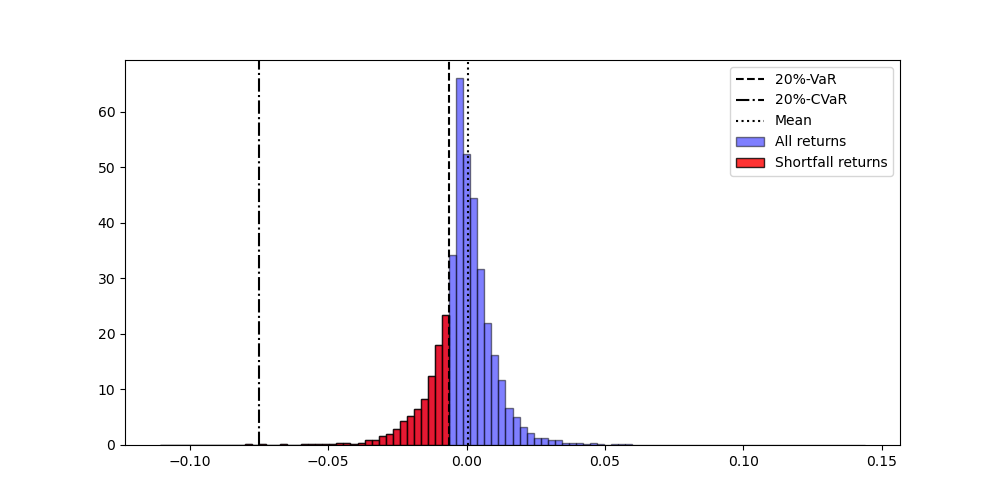
\includegraphics[width=1.0\textwidth]{./images/cvar_sp500_example.png}
        \caption{Conditional Value at Risk of S\&P 500 Daily Returns since 1993-02-01}
    \end{figure}
\end{frame}

\section{Neural Networks}

\begin{frame}
    \frametitle{Feed Forward Networks}
    For $d_i, d_h, d_o \in \N$
    and activation function $\sigma$,
    we define a single hidden layer \textbf{feed forward network} (FFN) as
    \[
        \text{FFN}_{W_2, b_2, W_1, b_1}^{d_i, d_h, d_o} : \R^{d_i} \to \R^{d_o}, \;
        x \mapsto W_2 \cdot \sigma (W_1 \cdot x + b_1) + b_2.
    \]
    Where
    \begin{itemize}
        \item $d_i, d_h, d_o$ are the dimensions of the input, hidden and output layer respectively,
        \item $W_1 \in \R^{d_h \times d_i}, W_2 \in \R^{d_o \times d_h}$ are weight matrices and
        \item $b_1 \in \R^{d_h}, b_2 \in \R^{d_o}$ are bias vectors.
    \end{itemize}
    We shorten the parameters and write $\text{FFN}_\theta^{d_i, d_h, d_o}$.
\end{frame}

\begin{frame}
    \frametitle{Common Activation Functions}
    \begin{figure}
        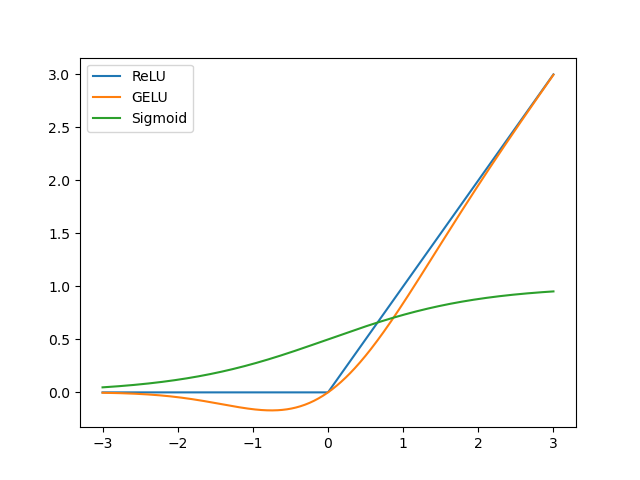
\includegraphics[width=0.8\textwidth]{./images/activation_functions.png}
        \caption{Common Activation Functions}
    \end{figure}
\end{frame}

\subsection{Universal Approximation Theorem}

\begin{frame}[t]
    \frametitle{Universal Approximation Theorem}
    Let $\sigma$ be non-constant and bounded, $d \in \N$
    and $\cNN_\infty := \{ \text{FFN}_{\theta}^{d, L, 1} \; | \; L \in \N \}$
    be the set of FFNs with arbitrary hidden layer size.
    Then we have: \\ \vs
    \begin{enumerate}
        \only<1->{
        \item For any finite measure $\mu$ on $(\R^{d}, \cB(\R^{d}))$
              and $p \in [1, \infty)$, the set $\cNN_\infty$ is dense in
              $L^p (\R^{d}, \mu)$.
              }
              \only<2->{
        \item If further $\sigma$ is continuous
              then $\cNN_\infty$ is dense in $C(\R^{d})$ in the sense that
              for any $f \in C(\R^{d})$ there exists a sequence of
              neural networks $\varphi_n \in \cNN_\infty$ that converges
              uniformly on any compact set $K \subset \R^{d}$ to $f$.
              }
    \end{enumerate}
    \only<2>{
        \vs The Universal Approximation Theorem goes back to
        \cite{nn_function_approximators}.
    }
    \only<3>{
        \vs Therefore, we may approximate any $\delta \in \H$
        arbitrarily well using a FFN.
    }
\end{frame}

\section{Deep Hedging}

\subsection{Heston Model}

\begin{frame}
    \frametitle{Heston Model}
    \begin{definition}[Heston Model]
        \only<1>{
            In a Heston model, the dynamics of the underlying risky asset $S$ are given
            by
        }
        \begin{align*}
            dS_t & = \mu S_t dt + \sqrt{V_t} S_t dB_t             \\
            dV_t & = \alpha (b - V_t) dt + \sigma \sqrt{V_t} dW_t
        \end{align*}
        \only<1>{
            where $B, W$ are two correlated Brownian motions with
            correlation $\rho \in [-1, 1]$.
        }
        \only<2>{
            \vs
            In our case, we are modeling a `typical equity market' using
            $$S_0 = 100, \alpha = 1, b = V_0 = 0.04, \rho = -0.7, \mu = 0 \text{ and } \sigma = 2.$$
        }
    \end{definition}
\end{frame}

\begin{frame}[t]
    \frametitle{GBM vs Heston}
    \begin{figure}[t]
        \centering
        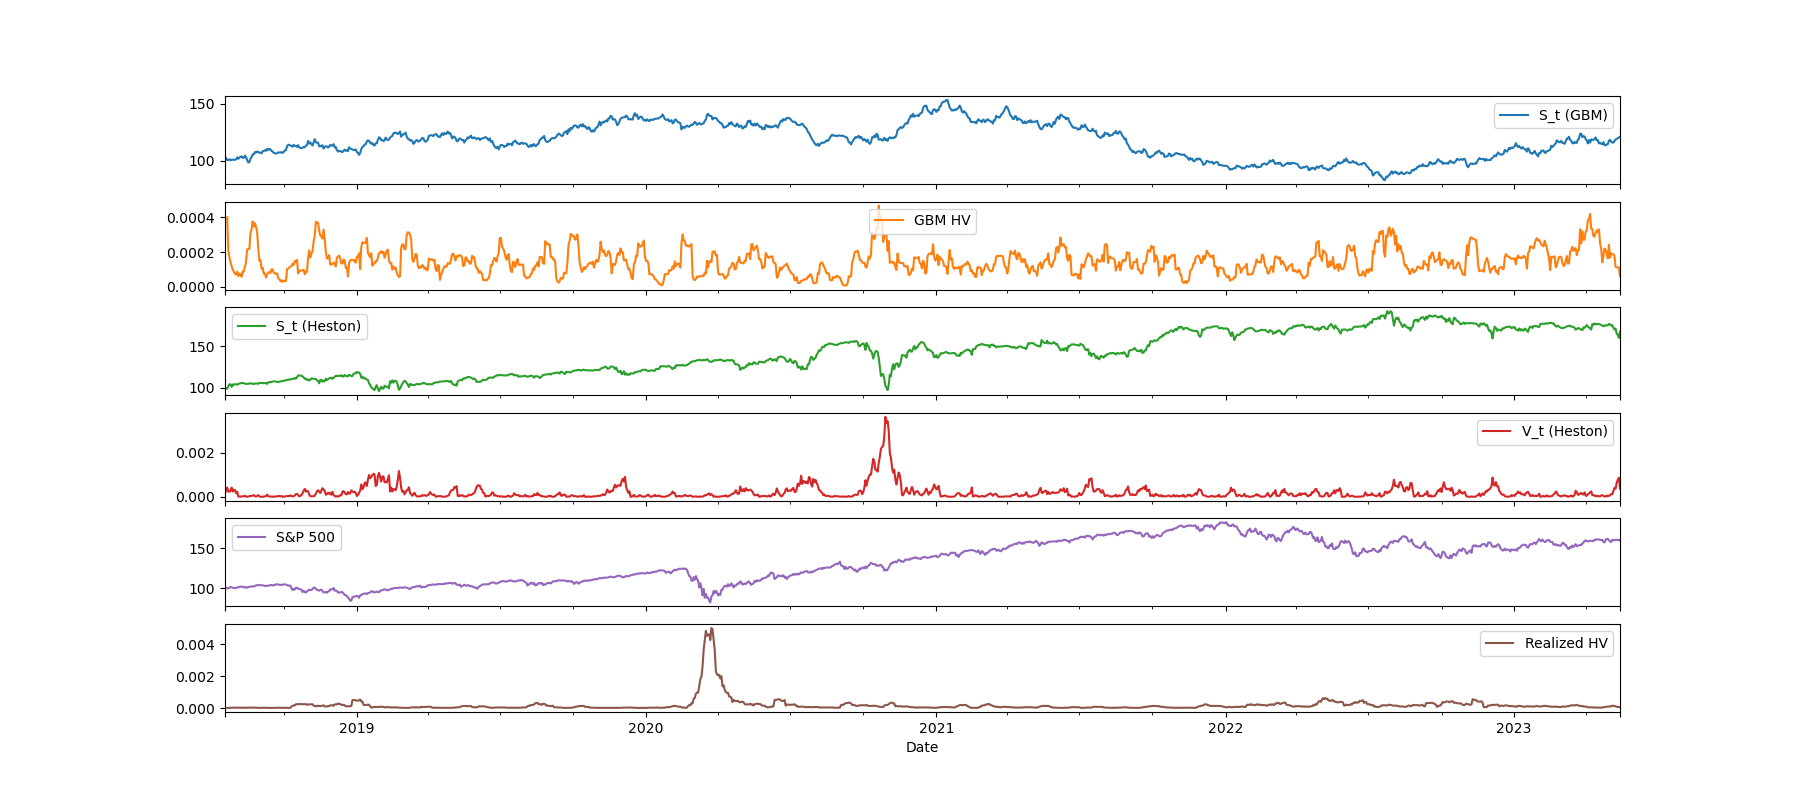
\includegraphics[width=1.0\textwidth]{./images/gbm_heston_example.png}
        \caption{
            Simulated stock prices by GBM and Heston as well as the real S\&P 500;
            Below each price we can see the corresponding (14 days rolling) volatility.
        }
    \end{figure}
\end{frame}

\subsection{Deep Hedging as Presented in The Paper}

\begin{frame}
    \frametitle{Idealized Variance Swap}
    In the paper, the hedging agent is allowed to trade in
    \begin{itemize}
        \item $S^{(1)}_t$, the underlying risky asset and
        \item an idealized variance swap which is defined as
              \begin{align*}
                  S^{(2)}_t & := \E_{\mathbb{Q}} \Big [
                      \int_0^T V_s \; ds \; \Big | \; \cF_t
                  \Big ]                                \\
                            & = \int_0^t V_s \; ds
                  + \underbrace{
                      \frac{V_t - b}{\alpha} (
                      1 - e^{-\alpha(T-t)}
                      ) + b(T-t)
                  }_{:= L(t, V_t)}.
              \end{align*}
    \end{itemize}
\end{frame}

\begin{frame}
    \frametitle{How this looks like}
    \begin{figure}
        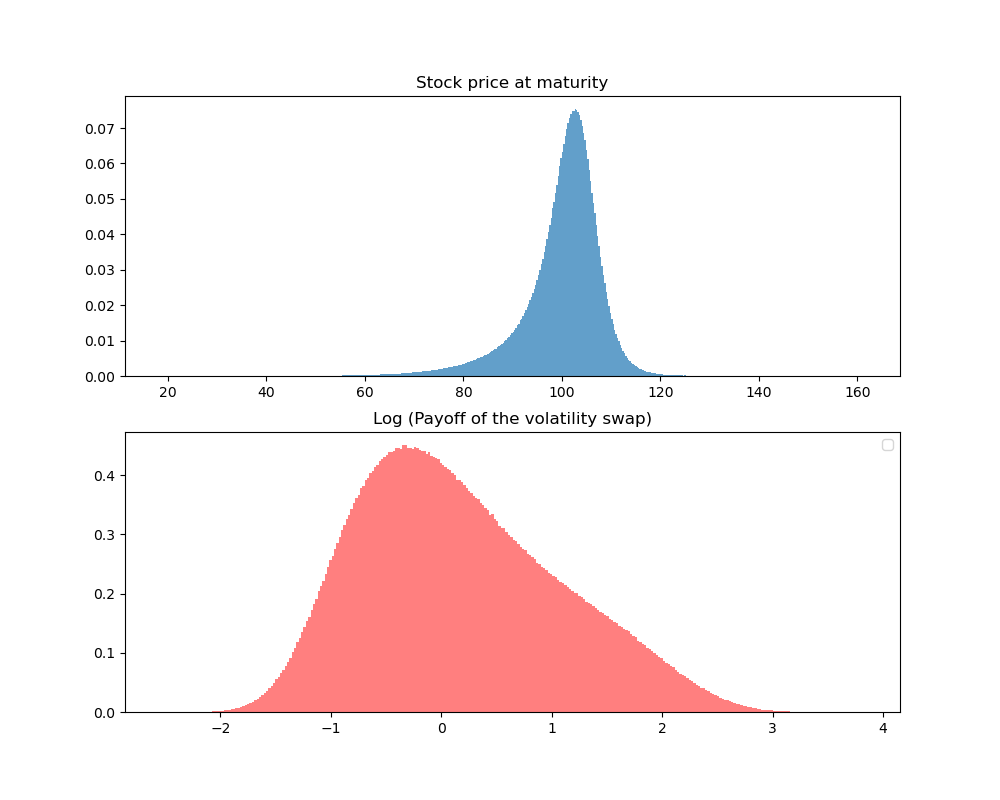
\includegraphics[width=0.7\textwidth]{./images/vol_swap_payoff.png}
        \caption{
            Histograms from $10^7$ simulations
            of $S^{(1)}_T$ and $S^{(2)}_T$ in the Heston model
            for $T=30$
            and parameters as in the paper
        }
    \end{figure}
\end{frame}

\begin{frame}
    \frametitle{How this looks like}
    \begin{figure}
        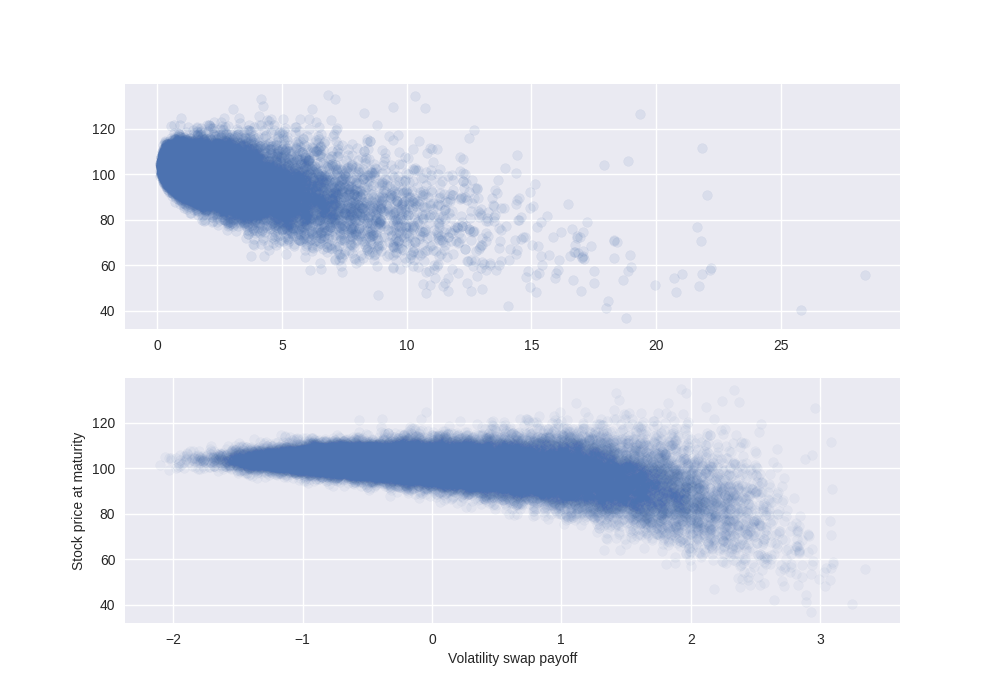
\includegraphics[width=0.8\textwidth]{./images/vol_swap_scatter.png}
        \caption{
            Scatter plot showing how $S_T$ and volatility swap
            payoff (or log thereof in the bottom plot) interact
        }
    \end{figure}
\end{frame}

\begin{frame}
    \frametitle{How this looks like}
    \begin{figure}
        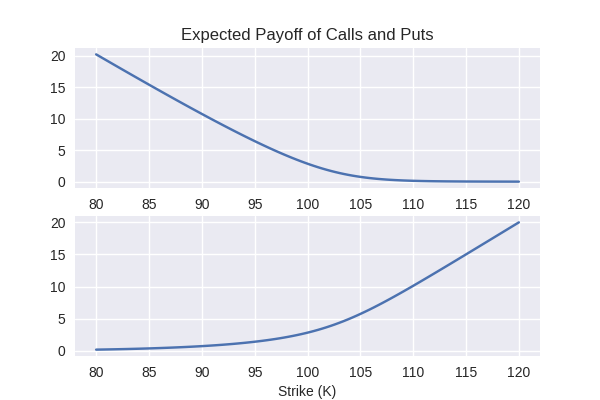
\includegraphics[width=0.7\textwidth]{./images/call_put_payoff.png}
        \caption{
            Expected Payoffs from Calls and Puts at $T=30$ with strikes
            on the x-Axis; Assuming $r=0$, these are the `fair' option prices
        }
    \end{figure}
\end{frame}

\begin{frame}
    \frametitle{How this looks like}
    \begin{figure}
        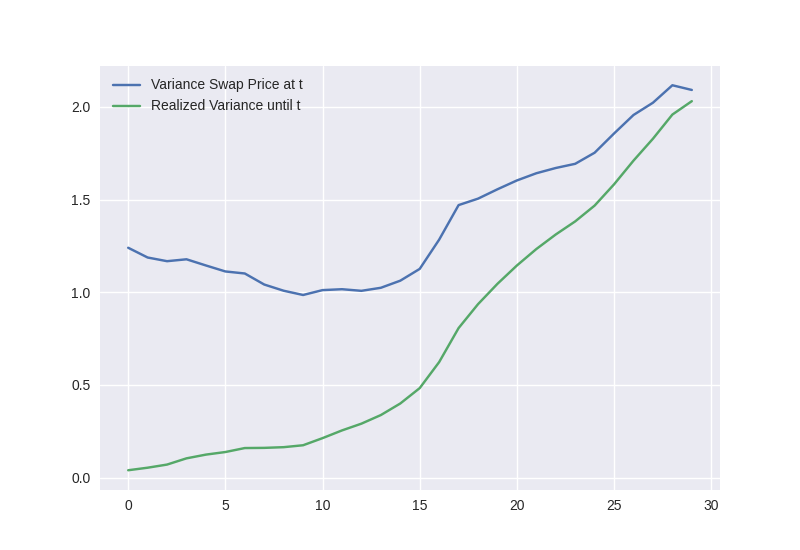
\includegraphics[width=0.7\textwidth]{./images/var_swap_price1.png}
        \caption{
            Price of a variance swap throughout a hedging period
        }
    \end{figure}
\end{frame}

\begin{frame}
    \frametitle{How this looks like}
    \begin{figure}
        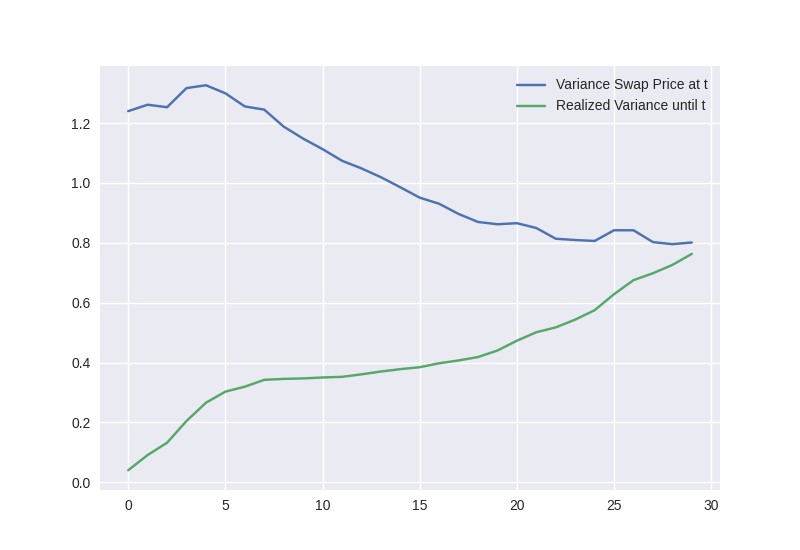
\includegraphics[width=0.7\textwidth]{./images/var_swap_price.png}
        \caption{
            Price of a variance swap throughout a hedging period
        }
    \end{figure}
\end{frame}

\subsection{Hedging using Deep Neural Networks}

\begin{frame}
    \frametitle{Learning Hedging Strategies}
    \begin{definition}[Information Set]
        Let $I_t$ be the $\F$-adapted information
        set with all the information we want to provide our
        hedging agent with. \\ \vs
        In our case, let
        \[
            I_t := (S^{(1)}_t, S^{(2)}_t)
        \]
        since our market model is \emph{markovian}.
    \end{definition}
    \only<2>{
        We may also allow additional information to be included
        in $I_{t-1}$, like upcoming earnings or market sentiment
        if such information can be built into our model somehow.
    }
    \only<3>{
        When hedging in a \emph{non-markovian} market, we might want to define
        \[
            \tilde{I}_t := (
            S^{(1)}_t, S^{(2)}_t, S^{(1)}_{t-1}, S^{(2)}_{t-1}, \dots, S^{(1)}_0, S^{(2)}_0
            ).
        \]
    }
\end{frame}

\begin{frame}
    \frametitle{Learning Hedging Strategies}
    \begin{definition}[Deep Hedging Strategy]
        For $L \in \N, d \in \N$, $\sigma: \R \to \R$
        an activation function,
        $I_t$ our information set at time $t$ and
        $\text{FFN}_\theta^{d+k, L, d} : \R^{d+k} \to \R^d$,
        a feed forward neural network, we define
        our \textbf{deep hedging strategy} as
        \begin{align*}
            \delta^\theta_t:
            \;\; & \R^{d+k} \to \R^d                                   \\
            I_{t-1} \mapsto \delta^\theta_t (I_{t-1})
                 & := \text{FFN}_\theta^{d+k, L, d} (I_{t-1})          \\
                 & = W_2 \cdot \sigma (W_1 \cdot I_{t-1} + b_1) + b_2.
        \end{align*}
    \end{definition}
\end{frame}

\begin{frame}
    \frametitle{Learning Hedging Strategies}
    Observe how our previous optimzation problem
    \[
        \pi (-Z) := \inf_{\delta \in \H} \rho (
        -Z + (\delta \cdot S)_T - C_T (\delta)
        )
    \]
    becomes, for $\delta^\theta \in \H$,
    \[
        \pi (-Z) := \inf_{\theta \in \Theta} \rho (
        -Z + (\delta^\theta \cdot S)_T - C_T (\delta^\theta)
        )
    \]
    % TODO: For OCE risk measures
\end{frame}

% TODO: Gradient Descent
% TODO: Randomness in the Gradient

\subsection{Pricing using Deep Hedging}
\subsection{Why Use Neural Networks?}

% And make the references slide using bibtex
\section{References}
\begin{frame}
    \frametitle{References}
    \bibliographystyle{apalike}
    \bibliography{references}
\end{frame}

\end{document}
